\begin{appendices}
\appendixpage
\noappendicestocpagenum
\addappheadtotoc

\chapter{Glossary}
\label{appendix:glossary}
\begin{multicols}{2}
\begin{itemize}
  \item CAVE : Cave Automatic Virtual Environment
  \item CoP : Center of Projection
  \item CSCW : Computer Supported Collaborative Work
  \item CVE : Collaborative Virtual Environment
  \item DLP : Digital Light Processing
  \item DoF : Degree of Freedom
  \item HCI : Human Computer Interaction
  \item HMD : Head Mounted Display
  \item IVE : Immersive Virtual Environment
  \item KS  : Kinematic State
  \item LC  : Liquid Cristal
  \item LCD : Liquid Crystal Display
  \item LoD : Level of Detail
  \item IPD : Interpupillary Distance
  \item IPT : Immersive Projected Technology
  \item SHC : Social Human Communication
  \item TSI : Transformed Social Interaction
  \item UML : Unified Modeling Language
\end{itemize}
\end{multicols}

\chapter{Test Platform - EVE}
\label{appendix:platform}
All experiments were carried out within EVE system (Evolutive Virtual Environment\footnote{http://www.limsi.fr/venise/EVEsystem}) using Virtools\footnote{http://www.3dvia.com/products/3dvia-virtools/} and BlenderVR \citep{BlenderVR2015}. It is a large CAVE-like system designed to provide multi-user and multi-sensorimotor perceptions in a large immersive virtual environment ($4.8m\times2.7m\times4.7m$) (Figure~\ref{fig:EVE}). The visual display of EVE system is composed of three screens surrounding a floor screen. Stereoscopic images are retro-projected on all these screens. Double-stereoscopy is provided on a combination of active and passive separation technologies, generating independent stereoscopic views for two users.

\begin{figure}[tb]
  \centering
  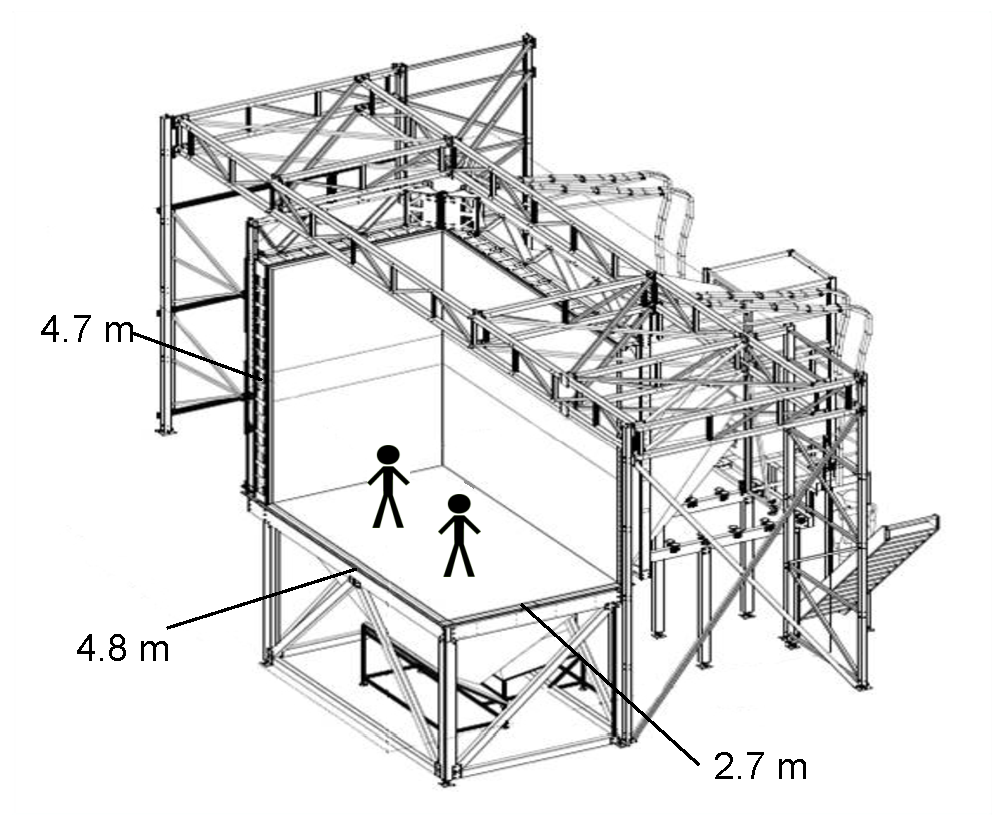
\includegraphics[width=0.7\textwidth]{figures/app/EVE}
  \caption{\label{fig:EVE}The Evolutive Virtual Environment (screen on the right-hand side is not shown in the figure).}
\end{figure}

This CAVE is equipped with a tracking system composed of infrared cameras to track user's motion. Markers installed on the shutter stereo glasses give us the information about the (head) position and orientation of the user so that adaptive stereoscopic images are computed for each user. Additional trackers - ART-Human Body Tracking Suit\footnote{http://www.ar-tracking.com} (Figure~\ref{fig:mocap}) are used for motion capture to enable full body interaction.

\begin{figure}[tb]
  \centering
  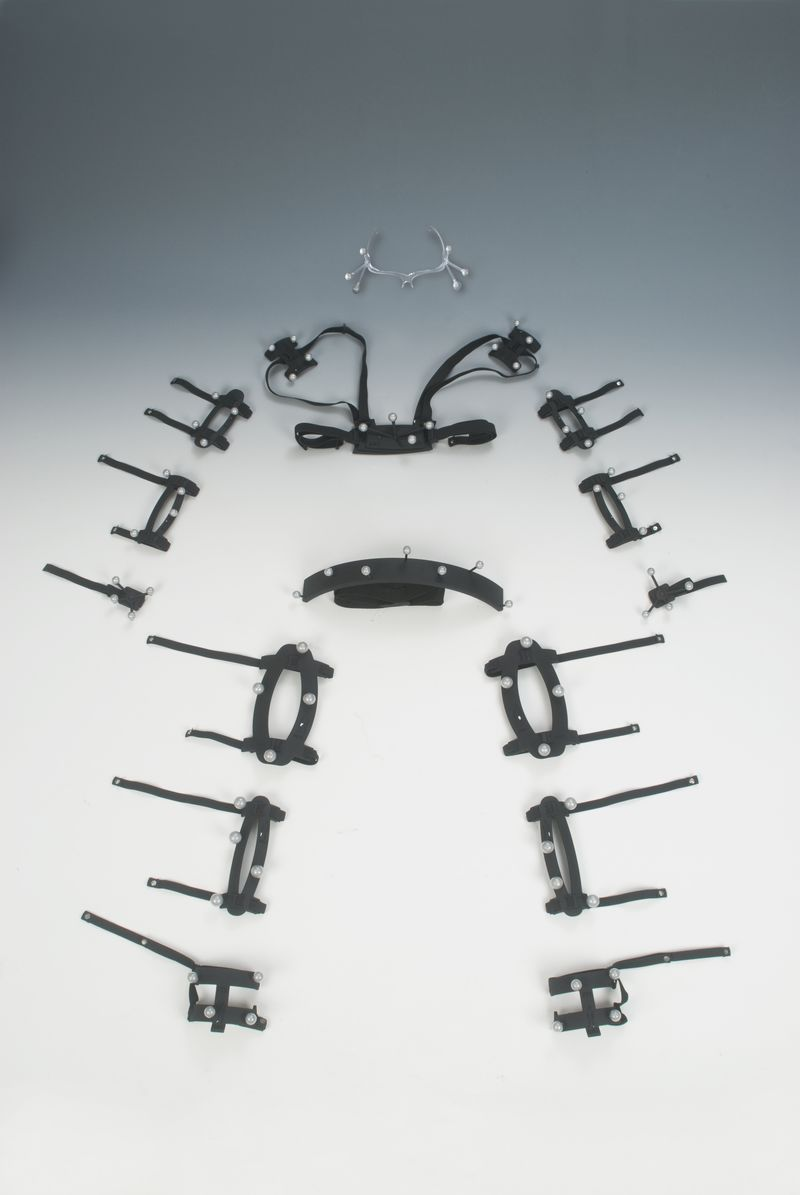
\includegraphics[width=0.4\textwidth]{figures/app/Mocap}
  \caption{\label{fig:mocap}The ART-Human Body Tracking Suit by Advanced Realtime Tracking GmbH.}
\end{figure}

\chapter{Dual-Presence Questionnaire}
\label{appendix:dual_pres_q}
The subjective questionnaire used in the experiment had a 4-point rating scale, ranging from 0 (do not agree at all), 1 (do not agree), 2 (neutral), 3 (agree), to 4 (fully agree). We regrouped the items into three categories according to three measured dimensions. Nine items measured the participant's feeling about his/her confidence on the success of collaborative task, 11 items estimated the participant's understanding of instructions, and 15 items measured participant's ease of dual-presence of the two forms of the collaborator.

\begin{enumerate}
	\item I succeeded in the task.
	\item I quickly identified the targets.
	\item I was rarely mistaken.
	\item I understood all the instructions.
	\item It was hard to follow the instructions.
	\item I easily identified the targets.
	\item The instruction didn't allow me to identify the target to be reached.
	\item I chose targets randomly.
	\item I wasn't always sure of myself in the choice of target.
	\item I had the impression that it was always the same target that was indicated by the instruction.
	\item I felt confused during the experiment.
	\item I preferred the instructions that were given only in verbal form.
	\item Some instructions were ambiguous.
	\item Some instructions didn't have a solution.
	\item I forgot the physical presence of the assistant.
	\item I only interacted with the virtual assistant.
	\item The physical presence of the assistant disturbed me.
	\item The physical presence of the assistant led me into mistakes.
	\item When the instruction indicated ``go to the crown on my left", I didn't understand which left was referred by the instruction.
	\item When the instruction indicated ``go to the crown on my right", I considered it as the right of the virtual assistant.
	\item When the instruction indicated ``go to the crown on my left", Sometimes I chose the left side of the virtual assistant and sometimes the left side of the real assistant.
	\item The instruction ``go to the crown on my left" has never been a problem to me.
	\item I tried to put myself in the position of the virtual assistant to understand the instruction ``go to the crown on my left".
	\item I can understand the instruction better when the assistant pointed to a target with a gesture without specifying whether it was on her left or right.
	\item During the experiment, I wasn't bothered by the physical presence and the virtual presence of the assistant.
	\item I would prefer that the assistant who helped me in the task wasn't physically present in the display system.
	\item I wasn't bothered by the physical presence of the assistant.
	\item I found that the task was facilitated by the simultaneous presence of my real assistant and her avatar.
	\item The proximity of the real assistant and the virtual assistant (the avatar) bothered me.
	\item I prefer the situation in which the virtual assistant was far away from the real assistant.
	\item When the real assistant and virtual assistant were close to each other, I had more difficulties to identify the target.
	\item I always paid my attention to the instructions given by the virtual assistant regardless of her position in the virtual scene.
	\item I had more trouble to rely on the virtual assistant when he/she was close to the real assistant.
	\item When the real assistant and the virtual one were far from each other, it was difficult for me to decide which target to choose.
	\item When the virtual and real assistants were combined (superimposed, both at the same location), I understood the instruction better.
\end{enumerate}

\chapter{Cohabitation Questionnaire}
\label{appendix:cohab_q}
A light-weight questionnaire for evaluating user cohabitation:
\begin{enumerate}
	\item I felt that I could collide my partner.
	\item I felt that I could collide the screens.
	\item I was afraid that my partner would collide me.
	\item I was disturbed by my partner when I moved around.
	\item My vision of the virtual scene was disrupted by my partner.
	\item I was aware of the movements of my partner next to me.
	\item I paid attention to my partner while performing my task.
\end{enumerate}

\chapter{Publications By the Author}

\begin{itemize}
\item \textbf{Weiya Chen}, Nicolas Ladeveze, C\'eline Clavel, Daniel Mestre, Patrick Bourdot. User Cohabitation in Multi-stereoscopic Immersive Virtual Environment for Individual Navigation Tasks. In \emph{Proceedings of IEEE Virtual Reality 2015}, in press.
\end{itemize}

\end{appendices}